%% LyX 2.1.4 created this file.  For more info, see http://www.lyx.org/.
%% Do not edit unless you really know what you are doing.
\documentclass[12pt,american,pointlessnumbers, abstracton, headsepline]{scrreprt}
\renewcommand{\familydefault}{\sfdefault}
\usepackage[T1]{fontenc}
\usepackage[latin9]{inputenc}
\usepackage{geometry}
\geometry{verbose,tmargin=2.5cm,bmargin=3.5cm}
\pagestyle{plain}
\setlength{\parskip}{\medskipamount}
\setlength{\parindent}{0pt}
\usepackage{array}
\usepackage{multirow}
\usepackage{amsmath}
\usepackage{amsthm}
\usepackage{graphicx}
\usepackage{setspace}
\usepackage{nomencl}
% the following is useful when we have the old nomencl.sty package
\providecommand{\printnomenclature}{\printglossary}
\providecommand{\makenomenclature}{\makeglossary}
\makenomenclature
\setstretch{1.2}

\makeatletter

%%%%%%%%%%%%%%%%%%%%%%%%%%%%%% LyX specific LaTeX commands.
%% Because html converters don't know tabularnewline
\providecommand{\tabularnewline}{\\}

%%%%%%%%%%%%%%%%%%%%%%%%%%%%%% User specified LaTeX commands.
% verschieden Symbole, Zeichen wie (c), �
\usepackage{textcomp,units}

% Mehr Platz zwischen Tabelle und Untertitel
\usepackage{caption}
\captionsetup[table]{skip=10pt}

%Kapitelzahl sehr gro�
\makeatletter% siehe De-TeX-FAQ 
 \renewcommand*{\chapterformat}{% 
   \begingroup% damit \unitlength-�nderung lokal bleibt 
     \setlength{\unitlength}{1mm}% 
     \begin{picture}(10,10)(0,5) 
       \setlength{\fboxsep}{0pt} 
       %\put(0,0){\framebox(20,40){}}% 
       %\put(0,20){\makebox(20,20){\rule{20\unitlength}{20\unitlength}}}% 
       \put(10,15){\line(1,0){\dimexpr 
           \textwidth-20\unitlength\relax\@gobble}}% 
       \put(0,0){\makebox(10,20)[r]{% 
           \fontsize{28\unitlength}{28\unitlength}\selectfont\thechapter 
           \kern-.05em% Ziffer in der Zeichenzelle nach rechts schieben 
         }}% 
       \put(10,15){\makebox(\dimexpr 
           \textwidth-20\unitlength\relax\@gobble,\ht\strutbox\@gobble)[l]{% 
             \ \normalsize\color{black}\chapapp~\thechapter\autodot 
           }}% 
     \end{picture} % <-- Leerzeichen ist hier beabsichtigt! 
   \endgroup 
}

\usepackage{ %a4wide,
            ellipsis, fixltx2e, mparhack,   %Fehlerkorrektur f�r Marginalien
            booktabs, longtable             %sch�nere Tabellen
}  

\usepackage[automark]{scrpage2}
%\automark[chapter]{chapter}
\clearscrheadfoot
\ohead{\\\headmark}
\ihead{\includegraphics[scale=0.15]{logo.jpg}}%\pagemark}
\ofoot[\pagemark]{\pagemark}


%Kurzfassung und Abstract (englisch) auf eine Seite
\renewenvironment{abstract}{
    \@beginparpenalty\@lowpenalty
      \begin{center}
        \normalfont\sectfont\nobreak\abstractname
        \@endparpenalty\@M
      \end{center}
}{
    \par
}



% sch�nerer Blocksatz!!
\usepackage{microtype}

\usepackage{ifpdf} % part of the hyperref bundle
\ifpdf % if pdflatex is used

%set fonts for nicer pdf view
 \IfFileExists{lmodern.sty}{\usepackage{lmodern}}
  {\usepackage[scaled=0.92]{helvet}
    \usepackage{mathptmx}
    \usepackage{courier} }
\fi

 % the pages of the TOC are numbered roman
 % and a pdf-bookmark for the TOC is added
 \pagenumbering{roman}
 \let\myTOC\tableofcontents
 \renewcommand\tableofcontents{
   %\pdfbookmark[1]{Contents}{}
   \myTOC
   \clearpage
   \pagenumbering{arabic}}

%Bezeichungen anpassen
%Babelpaket mu� zuvor geladen werden
%\usepackage[english]{babel}
%\addto\captionsngerman{} 
%\renewcommand{\figurename}{Abb.}% 
%\renewcommand{\tablename}{Tab.}% 
%\renewcommand{\abstractname}{Summary}
%\renewcommand{\nomname}{Abk�rzungen}


% Alle Querverweise und URLs als Link darstellen
% In der PDF-Ausgabe
 \usepackage[colorlinks=true, bookmarks, bookmarksnumbered, bookmarksopen, bookmarksopenlevel=1,
  linkcolor=black, citecolor=black, urlcolor=blue, filecolor=blue,
  pdfpagelayout=OneColumn, pdfnewwindow=true,
  pdfstartview=XYZ, plainpages=false, pdfpagelabels,
  pdfauthor={LyX Team}, pdftex,
  pdftitle={LyX's Figure, Table, Floats, Notes, and Boxes manual},
  pdfsubject={LyX-documentation about figures, tables, floats, notes, and boxes},
  pdfkeywords={LyX, Tables, Figures, Floats, Boxes, Notes}]{hyperref}

%mehr Platz zwischen �berschrift und Tabelle
\newcommand{\@ldtable}{}
\let\@ldtable\table
\renewcommand{\table}{ %
                 \setlength{\@tempdima}{\abovecaptionskip} %
                 \setlength{\abovecaptionskip}{\belowcaptionskip} %
                 \setlength{\belowcaptionskip}{\@tempdima} %
                 \@ldtable}

%In dieser Arbeit wird auf die Nomenklatur als Abk�rzungsverzeichnis verzichtet. Bei Wunsch wieder aktivieren.
%Nomenklatur als Abk�rzungsverzeichnis verwenden
%\renewcommand{\nomname}{Abk�rzungsverzeichnis}
%\renewcommand{\nomlabelwidth}{20mm}

%Nomenklatur als Glossar verwenden
%Nur Noetig wenn auch Glossar verwendet wird.
%\renewcommand{\nomname}{Glossary}

%Farbe f�r Programmcode festlegen
%\definecolor{lightgray}{rgb}{0.8,0.8,0.8}

\AtBeginDocument{
  \def\labelitemiii{\(\circ\)}
}

\makeatother

\usepackage{babel}
\begin{document}
\noindent \titlepage

\noindent \begin{center}
\begin{tabular}{cc}
 & \multirow{5}{*}{
\includegraphics{images/Logo_Uni_Kassel}}\tabularnewline
{\large{}Faculty Elektrotechnik / Informatik}\hspace{2.5cm} & \tabularnewline
 & \tabularnewline
 & \tabularnewline
 & \tabularnewline
\end{tabular}
\par\end{center}

\noindent \vspace{7cm}


\noindent \begin{flushleft}
\textbf{\Large{}Master Thesis}
\par\end{flushleft}{\Large \par}

\noindent \begin{flushleft}
{\large{}Homework Manage System with Git-Support and hierarchical
File database for Data management}
\par\end{flushleft}{\large \par}

\noindent \begin{flushleft}
{\Large{}\vspace{1.5cm}
}
\par\end{flushleft}{\Large \par}

\begin{tabular}{ll}
Submitted by:\hspace{1cm} & Hao Gao\tabularnewline
 & Matriculation number: 33101387\tabularnewline
 & \tabularnewline
 & \tabularnewline
 & \tabularnewline
Supervised by: & Prof. Dr. Albert Z�ndorf\tabularnewline
 & Universit�t Kassel\tabularnewline
 & Prof. Dr. Gerd Stumme\tabularnewline
 & Universit�t Kassel\tabularnewline
 & \tabularnewline
\multicolumn{2}{l}{Kassel, \today}\tabularnewline
\end{tabular}

\noindent \begin{flushleft}
\newpage{}
\par\end{flushleft}

~

\vspace{17.1mm}


\noindent \begin{flushleft}
\textbf{\huge{}Declaration of Authorship}
\par\end{flushleft}{\huge \par}

Deutsch oder English?

\vspace{2cm}


\noindent \begin{center}
\begin{tabular*}{15cm}{@{\extracolsep{\fill}}cl}
Kassel, \today & \tabularnewline
 & Hao Gao\tabularnewline
\end{tabular*}
\par\end{center}

\newpage{}

~

\vspace{17.1mm}


\noindent \begin{flushleft}
\textbf{\huge{}Summary}
\par\end{flushleft}{\huge \par}

zus�tzliche Zusammenfassung �ber Deutsch n�tig?

\newpage{}

\tableofcontents{}

\newpage{}



\pagenumbering{roman}
\setcounter{page}{7}

\listoffigures


\newpage{}

\listoftables


\newpage{}

\pagenumbering{arabic}


\chapter{Introduction}

motivation, why we need this kind of hms?


\chapter{Basics}

what were used in this project?explain the basics of the techniques


\section{techniques like framework and jpa?}

or?


\section{Related works}

moodle?


\chapter{Design}

The HMS is a web platform to manage the activities related to the
homework. In this chapter the detailed design of functions to support
the activities will be discussed.

The functions of the ''HMS'' system are divided into two parts.
The first part is to develop the common features which are similar
to other web platform,for instance ''register a user account'' .
The second part of the design is to develop the special core features
to distinguish the HMS system from other platform, the dynamic database
and the git based file management. 


\section{Common functions}

The main task of ''HMS'' is handling the process of handing in and
handing out the homework between the students and teachers. 
\begin{figure}[h]
\noindent \begin{centering}
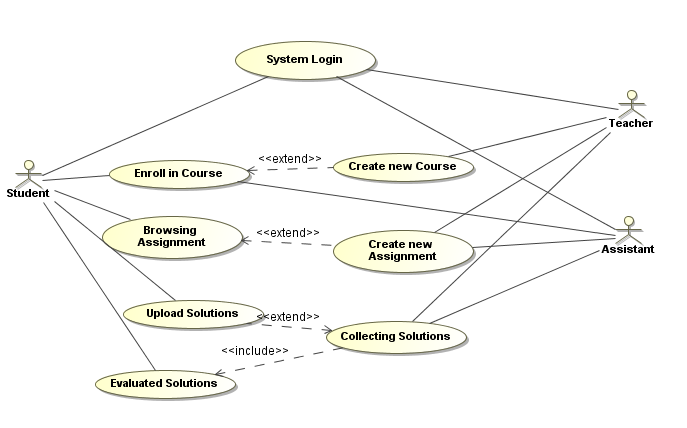
\includegraphics[scale=0.5]{images/generall}
\par\end{centering}

\caption{The use case from the perspective of different roll of user.\label{fig:The-use-case}}


\end{figure}
 

As the Figure \ref{fig:The-use-case} shows,there are several steps
within this process from the prospective of the user roll. First considering
the user roll of students,the student should be able to register a
account of ''HMS'', after logging into the system the students can
browsing all the available courses in the system and subscribing the
target course. Then it is possible for the students to view the homepage
of the course and download the available homework. and finally uploading
the solutions to the homework accordingly. the process of uploading
a homework to the system is finished at the student side. now take
a look at the side of Teacher and Assistant, besides the registration
and logging process, the user group of teacher can create new course
and new assignment also collecting the handed in homework and give
them back to the students once the evaluation is finished. The assistants
however can not creating new course, but should be able to add new
assignment and evaluate the handed in homework as well. In summary,
in order to realize the main task of the ''HMS'', the ''HMS''
system should have following capabilities:
\begin{enumerate}
\item User management including ''Registration'' , ''Role based access
control'',''Self management''.
\item Course management including ''Creation of Course'',''Modification
of Course''.
\item Assignment management including ''Creation of Assignment'',''Distribution
of Assignment'',''Collecting of Assignment'',''Evaluation of Assignment''.
\end{enumerate}
Besides the above listed capabilities, the HMS should also provide
a way that the students and teachers can communicate with each other.
firstly a private message system will be needed for the students and
teachers to exchange the information about the problem of assignment
or evaluations individually,also the new message system should work
as a instant message system,in this way the questions or the problems
between the students and teachers can resolve more efficiently. secondly,
a course forum is also not a bad idea, a common scenario is that more
students may have a same question for a new assignment, if a students
write a new post about this question, and the teacher gives a answer
to the question, the other students with the same question can also
get the answers and avoiding asking the same questions again. This
saves the time from both side. So the communications system for the
HMS has two parts:
\begin{enumerate}
\item Instant private message system.
\item a public course forum for each course.
\end{enumerate}

\subsection{User management}

The user management of the ''HMS'' system consists of several modules(Figure
\ref{fig:The-Modules-of-usermanagement}), first is the registration
module, with this module the user can use their email address to register
a account in HMS system. second is the self management module. after
the user has logged into the system, they should be able to change
their emails and password or other personal details.third is the user
role control module, this is necessary for system to arrange the proper
functions to the current user based on their user role, the user obtains
a startup role at the registration, later on the user role can be
changed by the system admin. In the rest of this section, all the
modules will be detailed discussed.

\begin{figure}[h]
\noindent \begin{centering}
\includegraphics{\string"images/module usermanagement\string".png}
\par\end{centering}

\caption{The Modules of user management\label{fig:The-Modules-of-usermanagement}}


\end{figure}



\subsubsection{a. Registration}

\begin{figure}[h]
\noindent \begin{centering}
\includegraphics[scale=0.6]{\string"images/Registration activity_cut\string".png}
\par\end{centering}

\caption{Registration activity\label{fig:Registration-activity}}
\end{figure}


Figure \ref{fig:Registration-activity} shows the workflow when a
user register a new account. the user first use the registration form
to fill in all the relevant information , for instance the password,
email, and students number, after clicking the sign up button, the
whole process begins, first the validation of the registration form
will be performed to check whether the user has fill in all the required
field and without error, if user passed the form validation, the HMS
system will then send a confirmation email with a confirmation URL
to the email address from the registration form, if the user click
the confirmation link, the user will be redirect to the website and
can directly starting using the account. Otherwise the user has to
start over the registration process. The step of email address confirmation
is important because this procedure allows the system to check that
the user actually signed up for the account and guarantee the email
of this user is valid and ready to receive the system information.


\subsubsection{b. Self Management}

\begin{figure}[h]
\noindent \begin{centering}
\includegraphics[scale=0.85]{\string"images/self management\string".png}
\par\end{centering}

\caption{The functions of self management\label{fig:The-functions-of-selfmanagement}}
\end{figure}


It is very common that user may forget their passwords or even worse
their registered email becomes invalid, so it is necessary to develop
the functions, user can use to reset their email and passwords. The
resetting of email address or the passwords works similar as registration.
If user choose to reset their email address, first they will be asked
to type in the new email address,after that user click the reset button,
the system should send a new confirmation email to the new address,
when user click the hyper link in the email, a new web page will be
generated and user can confirm the address change. if user choose
to reset their passwords, they just need to click the reset password
button, the system will send another confirmation email with a hyper
link, the user can use this link to type in their new passwords. Besides
the modification of passwords and email address,there is another function
should be added to self management, thus the HMS system use git server
to control all the homework files, and this git server use ssh to
authenticate the connections, the system should also provide a function
that user can add their ssh public key to the git server, so that
they can connect their computer direct to the git server. Figure \ref{fig:The-functions-of-selfmanagement}gives
a overview for all the components of the self management.


\subsubsection{c. Role based access control}

\begin{figure}[h]
\noindent \begin{centering}
\includegraphics[scale=0.85]{\string"images/user role\string".png}\caption{Different user role in HMS system\label{fig:Different-user-role}}

\par\end{centering}

\end{figure}


The user of the HMS system has different roles, and they need different
functions. for instance a teacher can create new course but students
can not, so it is important for the system to distinguish the user
based on their user roles, so that the system can serve different
functions to different user.

Figure \ref{fig:Different-user-role} shows all the user role in HMS
system,from the top is the system admin, the system admin account
will be generated at the first boot up of the HMS,the user name and
password of the system admin will be saved under the home directory
of the current server admin. it means only the admin of the server
can access the username and passwords of HMS system admin account,
this can ensure that only trusted personal can access the system admin
account of HMS.The job of system admin is to manage other user's role
and the system database(backup the database after semester ends).
At the bottom are the normal user roles. first is the default user,every
user obtains this role after registration.if you don't give a students
number.The user with this role can not do much things within the system
other than updating their email address or passwords. if the default
user wants to promote their user role to another level, they have
to contact system admin. second user role is students,if user register
the account with their students number, they will automatically obtain
a student account, with student account the user can browse all the
available course and join the course, download and upload homework,
using the communication system like chat and forum. third user role
is assistants, besides all the functions of students, assistants can
create new assignment and review all the handing in homework and make
a evaluation,last one is the teacher, the teacher account has all
the functions of assistant account and additionally the teacher can
also create new course.


\subsection{Course management}

There are two types of course for informatics students, in the first
type of course the students have to hand in various homework, and
the points gained from those homework are usually used as a prerequisite
for the final exam. in the second type of course the students will
get a semester assignment, normally a whole software project, the
points gained from this project usually is the final points for this
course. additionally every students will get a git repository after
user had signed up the course,this repository will also worked in
two modes according to the type of course,the details of git working
modes will be discussed in more detail.

\begin{table}[h]
\noindent \begin{centering}
\begin{tabular}{|c|>{\raggedright}p{6cm}|>{\raggedright}p{3cm}|>{\raggedright}p{3cm}|}
\hline 
Features & Precondition to final exam & Git repository Mods & Performance Evaluation\tabularnewline
\hline 
Type I & \begin{enumerate}
\item Students have to hand in at least amount of valid homework.
\item A valid homework requires normally for students to gain more than
50\% points of a assignment.
\item A student should gain at least 50\% of total points for final exam\end{enumerate}
 & Git repository works under local modus\\
(Student can only hand in the homeworks through course homepage) & need detail evaluation of assignments\\
(number of valid handin, percentage of gained points)\tabularnewline
\hline 
Type II & None,Students just need to hand in the final project & Git repository works under remote modus\\
(Student can use the course repository as any remote git repository) & Only final evaluation\tabularnewline
\hline 
\end{tabular}
\par\end{centering}

\caption{Features of different types of course\label{tab:Features-of-course}}
\end{table}


The Table \ref{tab:Features-of-course} shows the different features
of different types of course.The function of ''creating course''
should take all the features from above into consideration. 


\subsection{Assignment management}

\begin{figure}[h]
\noindent \begin{centering}
\includegraphics[scale=0.8]{\string"images/assignment management\string".png}
\par\end{centering}

\caption{Sequence diagram for assignment management\label{fig:Sequenz-diagram-for-assignment}}


\end{figure}


Figure \ref{fig:Sequenz-diagram-for-assignment} shows the sequence
of handing in and handing out a assignment, after creating a new course,
teacher can start adding assignments to the course, when a new assignment
has been successfully added to the course, the course homepage for
students will show this new assignment and with a download link, student
can download the assignment and start working on the new assignment.
later when students finished the assignment,the solution will be uploaded
to the according assignment and teacher can review them at the evaluation
part of the course's homepage and add a evaluation to the solution.
When the evaluation is successfully saved to the assignment, the student
will get the results directly at course homepage.


\subsection{Communication system}


\subsubsection{a. Forum}

The HMS system has a standard client-server structure, the client
and server communicate with each other over internet using HTTP protocol.\cite{daa}
HTTP has a typical ''Request-Response'' pattern, the web client
sends a request to the web server, web server serves a response according
to the web client request. It is a simple but powerful solution to
provide a two-way conversation for two party over one channel.\cite{Hohpe2012}
The forum function within the HMS system works also after this pattern,
Figure \ref{fig:Forum-message-pattern} shows the communication between
the clients and HMS server based on the different forum action request.for
instance: a client sends a ''create new post'' request to the server,
the HMS server accepts the request and save this new post to the related
course forum, and return the content of this post to the client again.

\begin{figure}[h]
\noindent \begin{centering}
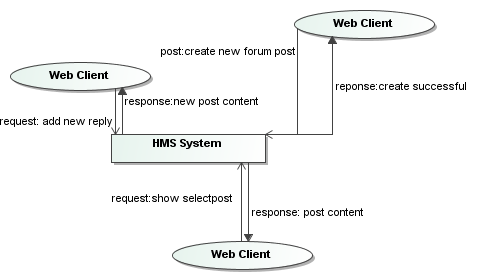
\includegraphics[scale=0.85]{images/forum}
\par\end{centering}

\caption{Forum message pattern\label{fig:Forum-message-pattern}}


\end{figure}



\subsubsection{b. Instant message}

The standard HTTP protocol however is not suited for the instant message
system, because of the ''Request-Response'' message pattern, user
has to manually ask for a content upgrade. But a instant message system
needs automatically update the chat contents on both side of a conversations
while a new message has been added\cite{day2000model}. therefore
a full-duplex communication system ''Web Socket''\cite{mozilla}will
be used to back up the message module. Figure \ref{fig:Websocket-message-pattern}
illustrate a simple use case of web socket,after logging into their
HMS account user A and user B are both connecting to the HMS web socket
server, later on user A send a new message to user B,first the request
from user A are passing to the web socket server,the server processed
the request accordingly and served the response not only to the user
A but also automatically served the response to the user B,this ensure
the both side of the conversation can have their message received
in real time.

\begin{figure}[h]
\noindent \begin{centering}
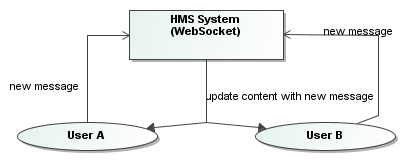
\includegraphics[scale=0.85]{images/message}
\par\end{centering}

\caption{Web socket message pattern\label{fig:Websocket-message-pattern}}


\end{figure}



\section{Specific functions}

The functions from last section needs two critical preconditions to
work:
\begin{enumerate}
\item The files of assignment and student's submissions can be saved.
\item The result of the activities can be persistent in a database.
\end{enumerate}
There are already plenty solutions to those problems,for instance
the file upload and the database support are the standard functions
within the play framework. The developer just need to decide where
to put the files and configure the configuration file for database
to work. However there are still some disadvantages with the standard
approach,this will be discussed in the rest of this section and the
new approaches for both will be introduced.


\subsection{Submission management}

The normal approach for the file upload in Play framework is pretty
simple,the developer only need to defined the extra file attribute
for a HTML form and send the form through POST methode of HTTP protocol,and
defined a java controller on the server side to save the file to a
desired location. Also if the user want to retrieve this file again,
the developer just need to save the path of this file under the name
of the user in a database. But when considering this file is a homework
submission,there is still need a lot work to do than just upload a
file to the server. The documentation of the moodle system has suggests
several submission type related to file submission\cite{documoodle}:
\begin{enumerate}
\item Student submit a work and teacher download it later.
\item Student submit a work multiple times.
\item Student submit a work with a response.
\end{enumerate}
The first type can direct use the default file upload function with
a database recording the file path. For second type there are two
ways to solve it, first way is that every time when students submit
a new version, the old version will be deleted, and teacher will always
get the latest version,the downside of this solution is that the previous
upload will be all gone,there is no way for teacher to track the submission
history. another is that when a new version is submitted,the old version
will not be deleted,however with this solution the teacher do can
track the history but will taken two much hard drive capacity.For
the last type it is just need to put a extra column in the database
to save the response with the file path. 

All these submission type can be solved just using the standard techniques.
But this is still too complicated, not only for development but also
for the user of the system. At this point the GIT will be introduced
to resolve the problem.

\begin{figure}[h]
\noindent \begin{centering}
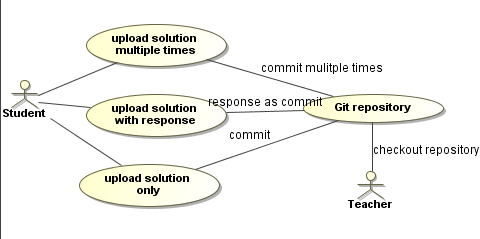
\includegraphics[scale=0.8]{images/git}
\par\end{centering}

\caption{Workflow of git\label{fig:Workflow-of-git}}


\end{figure}


Figure \ref{fig:Workflow-of-git} shows the workflow for this 3 type
of submission when using the git repository. Every students when they
join a course, they will automatically get a git course repository
from the system,all the submissions of the student will be written
into this repository. all this scenario from above can be solved just
using the git commit. no matter what submission type was chosen by
the students,the only difference how many commits were made. on the
teacher side they just need to checkout the students git repository
and read the commit history. naturally the repository address is also
needed to be saved into the database. 


\subsection{Database}

Play frameworks support several database engine:
\begin{itemize}
\item H2
\item SQLite
\item PostgreSQL
\item My SQL
\end{itemize}
only H2 and SQLite support the embedded mode,the embedded database
runs directly in the application that uses them,it requires no extra
server and no maintenance for the database itself.Another advantage
of embedded database is the speed, because all the database operations
happen inside the application process.\cite{Chaudhri2003}In this
project the H2 database engine will be used as the default database
engine. first h2 support the embedded mode and it is purely written
in java, the java API of h2 can be directly used in the play framework.
another reason is that the embedded database runs within the application,
it is normally hidden from the end user\cite{Chaudhri2003}, so there
is no way the user can side load the database, but in the real life
of maintaining the HMS system, direct accessing and manipulating the
database using a SQL query tool sometimes is more efficiency than
the usual routine.in this case h2 support a mixed mode(Figure \ref{fig:Mixed-Mode-of-h2}),mixed
mode is a combination of the embedded mode and server mode, the first
application (in this case the HMS) will use the database as embedded
mode, but it also starts a server so that the other application(a
SQL query tool) can still side load the database.It is also importent
to notice that if the application is shut down, the server mode will
also close all the connections\cite{h2database},therefore side loading
a database using remote mode can only take place when HMS is still
rung. However the database file generated by the h2 engine can still
be loaded with the h2 web based manage tools.

\begin{figure}[h]
\noindent \begin{centering}
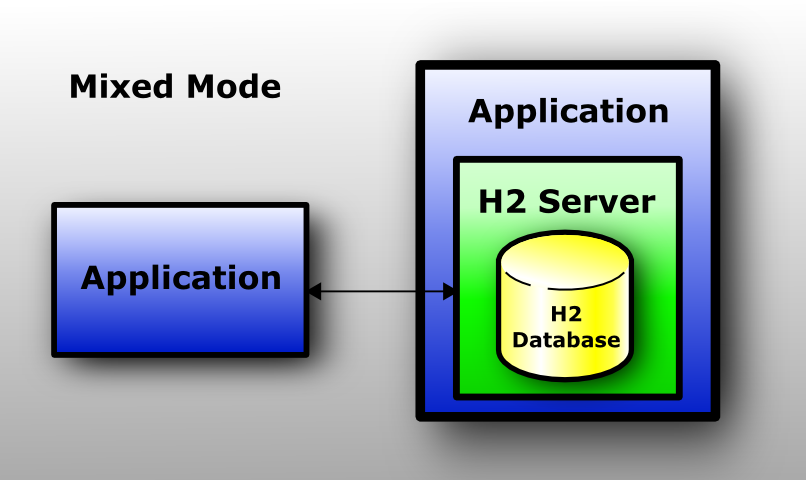
\includegraphics[scale=0.8]{images/connection-mode-mixed-2}
\par\end{centering}

\caption{Mixed Mode of h2 server\cite{h2database}\label{fig:Mixed-Mode-of-h2}}


\end{figure}


Play framework uses Ebean ORM to access the database,ORM is a technique
to convert objected oriented programming language(in this case Java)
into its persistence as a relational data base, so the data can freely
exchange between a java object and database table.\cite{K2009}By
default the configuration of Ebean and the database is done by editing
the configuration file of play framework. After configuration of the
database engine and the Ebean, the system is ready for developer to
design the database for the web application.

This is the standard approach when developing a web application using
play framework. But it also has a problem, the database configuration
has to be done before the application started, in the run time of
the application all the database related actions can only take place
within the preconfigured database. This approach is convenient for
the developer, because the developer don't need to take care of the
programmatically details of bring database ,ORM and application together.But
it sometimes cause trouble for the end user. Usually there will be
only one predefined database, all the data from the web application
will be saved within this database. In this project, HMS is designed
for managing the homework for teacher,and the system will be used
in a university,every once in a while the university need to archive
or backup the old data from the past term. A possible way is query
out all the related data based on the semester, then dump the data
into file and save the file some where else. Moodle also use this
approach to make a course backup\cite{moodlebackup}.The disadvantage
of this approach is strait forward,the amount of data will increasing
rapidly after years of use, it is not only complicated but also consume
a lot of time.

\begin{figure}[h]
\noindent \begin{centering}
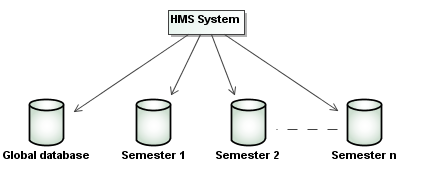
\includegraphics[scale=0.8]{images/database}
\par\end{centering}

\noindent \centering{}\caption{multiple database based on semester\label{fig:multiple-database}}
\end{figure}


Figure \ref{fig:multiple-database} shows a better approach used in
the HMS project. all the data can be separate saved on different database
based on the semester, the back up process will a lot easier.First
the data structure of every semester is the same, so the database
design for semester can be reused in every new semester,therefor no
need to query the data. second the database in this project working
under the embedded modes,all the relevant data of the database are
saved in a single file. so each semester will be a single file, backup
the semester data only need to copy the database file to some where
else.

aside from the semester data, there is a additional database to manage
all the data related to the authentication process, for instance the
email address,password,and ssh public keys. 

This approach requires the system to create a database in the run
time, therefore the standard database configuration of play framework
can not be used. The details of implementing the dynamic database
function will be demonstrated in the next chapter.


\chapter{Implementations}

how to implement the functions from chapter4


\section{User management}


\section{Course management}


\section{Assignment management}


\section{Communication system}


\section{Integration of Git}


\section{Database design}


\chapter{System usage}

Test run?


\section{First run}


\chapter{Evaluation}


\chapter{Summary and Outlook}

\clearpage
\phantomsection
\addcontentsline{toc}{chapter}{Glossary}

\nomenclature{HMS}{Homework Management System}\nomenclature{ORM}{Object-relational mapping}

\settowidth{\nomlabelwidth}{ORM}
\printnomenclature{}

\clearpage
\phantomsection

\bibliographystyle{bibtex-daten/unsrtdin}
\addcontentsline{toc}{chapter}{\bibname}\bibliography{bibtex-daten/bachelorarbeit-info}

\end{document}
